\section{Method}
Iterations have been:
\begin{itemize}
    \item Interpolated boundary conditions
    \item Linear interpolation
\end{itemize}

\todo{These sections are taken from the JASA appendix} In this appendix, some iterations done over the course of this project will be shown in more detail. In the following, the 1D wave equation with a wave speed of $c = 1470$ m/s, a length of $L = 1$ m, Dirichlet boundary conditions and a sample rate of $f_\text{s} = 44100$ Hz is considered, and -- through Eq. \eqref{eq:compactLambda} -- satisfies the CFL condition with equality. These values result in $N = 30$, or a grid of 31 points including the boundaries. Then, the wave speed is decreased to $c \approx 1422.6$ m/s, i.e., the wave speed that results in $N=31$ and satisfies the stability condition with equality again. 

\subsection{Full-Grid Interpolation}
One way to go from one grid to another is performing a full-grid interpolation \cite[Chap. 5]{theBible}. If the number of points changes according to Eq. \eqref{eq:orderOfCalcGrid}, i.e., if $N^n \neq N^{n-1}$ the full state of the system ($u_l^n, u_l^{n-1}\ \forall l$)  can be interpolated to the new state. See Figure \ref{fig:fullGrid}. 

\begin{figure}[ht]
    \centering

%% \reprintcolumnwidth is the same in preprint and reprint for
%% ease of use for authors:
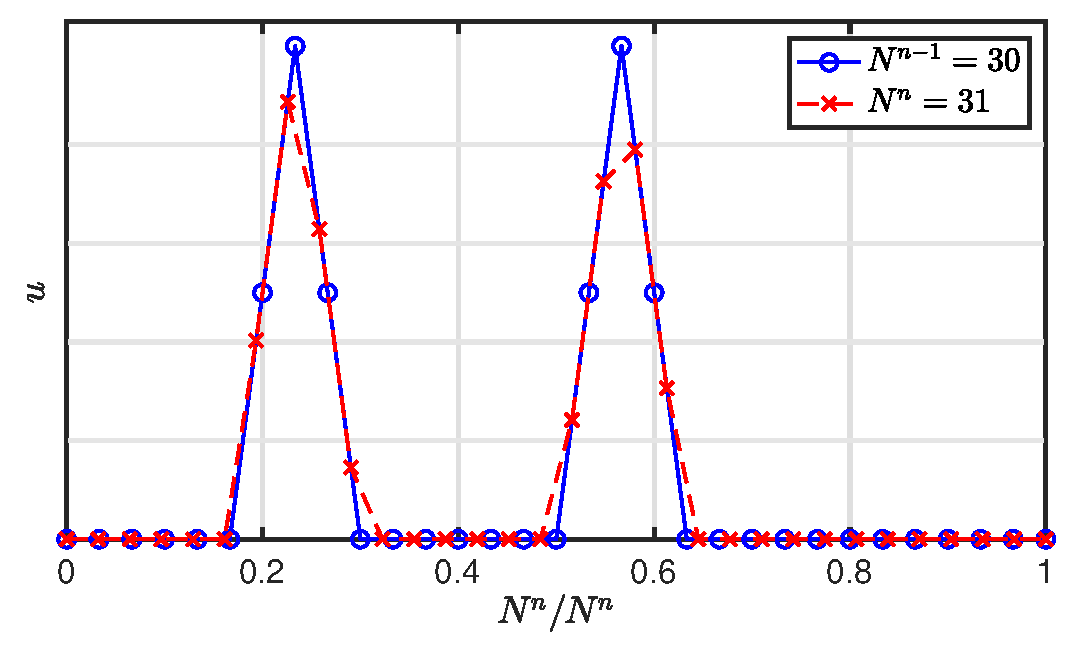
\includegraphics[width=0.5\textwidth]{dynamic/fullGrid.eps}
\caption{\label{fig:fullGrid}{Upsampling $u$ (with an arbitrary state) using (linear) full-grid interpolation with $N^{n-1} = 30$ and $N^n = 31$. The horizontal axis is normalised with respect to $N^n$.}}
\end{figure} 

An issue that arises using this method is that the Courant number $\lambda$ will slightly deviate from the CFL condition as $c$ changes. Using Eq. \eqref{eq:compactLambda} with $L/ck$ approaching $31$ (from below), the minimum value of $\lambda \approx 30/31 \approx 0.9677$.
%\footnote{Eq. \eqref{eq:orderOfCalcGrid} can be compactly rewritten as $\lambda = \frac{ck}{L}\cdot \text{floor}\left(\frac{L}{ck}\right)$. As $L/ck$ approaches $31$ (from below), $\lambda \approx \frac{30}{31}$.}
This, employing Eq. \eqref{eq:fmax}, has a maximum frequency output of $f_\text{max} \approx 18,475$ Hz. 
%For slightly lower values of $c$, $N = 31$ and $\lambda \approx 1$. 
The Courant number will deviate more for higher values of $c$ and thus lower values for $N$ -- for instance, if $N$ approaches $11$ (from below), $\lambda \approx 10/11 \approx 0.9091$ and $f_\text{max} \approx 16,018$ Hz.

Another problem with full-grid interpolation, is that it has a low-passing effect on the system state, and thus on the output sound. %Figure \ref{fig:fullGrid} shows the biggest changes are in the state are at the locations with the biggest difference between the states of consecutive grid points.
Furthermore, this state-interpolation causes artefacts or `clicks' in the output sound as the method causes sudden variations in the states.  

All the aforementioned issues could be solved by using a (much) higher sample rate and thus more grid points, but this would render this method impossible to work in real time.

\subsection{Adding and removing Points at the Boundary}\label{sec:addAtBoundary}
To solve the issues exhibited by a full-grid interpolation, points can be added and removed at a single location and leave most points unaffected by the parameter changes. A good candidate for a location to do this is at a fixed (Dirichlet) boundary. The state $u$ at this location is always $0$ so points can be added smoothly. 

As $c$ decreases, $h$ can be calculated according to Eq. \eqref{eq:orderOfCalcGrid} and decreases as well.

This has a physical analogy with tuning a guitar string. Material enters and exits the neck (playable part of the string) at the nut, which in discrete time means grid points appearing and disappearing at one boundary.

To yield smooth changes between grid configurations, an interpolated boundary has been developed, the possibility of which has been briefly mentioned in \cite[p. 145]{theBible}. The Dirichlet condition in Eq. \eqref{eq:contDirichlet} can be extended to be the simply supported boundary condition:
\begin{equation}
    u(x, t) = \frac{\partial^2}{\partial x^2}u(x, t) = 0 \quad \text{where} \quad x = 0, L,
\end{equation}
or, when discretised,
\begin{equation}\label{eq:simplySupportedDiscrete}
    u_l^n = \delta_{xx}u_l^n = 0, \quad \text{where} \quad l = 0, N.
\end{equation}
This means that on top of that the state of the boundary should be $0$, the curvature around it should also be $0$. One can again solve for the virtual grid points at the boundary locations, yielding
\begin{equation}
    u_{-1}^n = -u_1^n \quad \text{and} \quad u_{N+1}^n = -u_{N-1}^n.
\end{equation}
This is visualised in Figure \ref{fig:simplySupportedBound}.

\begin{figure}
    \centering
    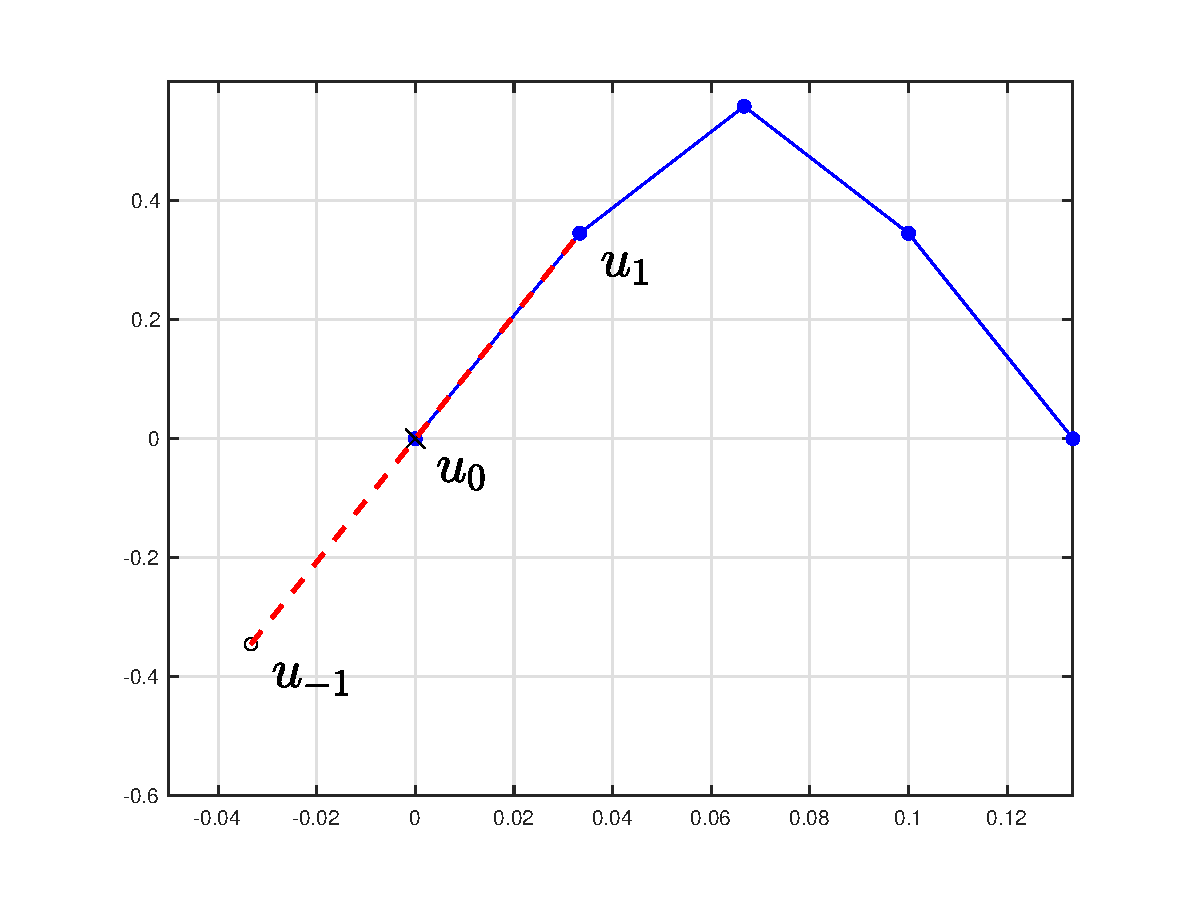
\includegraphics[width=0.7\textwidth]{dynamic/simplySupportedBoundary.eps}
    \caption{\label{fig:simplySupportedBound}{The simply supported boundary condition: both the state and the curvature at the boundary -- at $l=0$ -- should be $0$.}}
\end{figure} 

If the flooring operation in Eq. \eqref{eq:numberOfIntervals} is removed this introduces a fractional number of grid points.


The by-product of using a fractional $N$ this is that the CFL condition in \eqref{eq:CFL} can now always be satisfied with equality no matter what the wave speed is.

An issue with this method is that removing points is much harder than adding.

their interactions change through a change in the grid spacing and wave speed. This interaction, though, is defined by $\lambda$ which 

\begin{figure}
    \centering
%% \reprintcolumnwidth is the same in preprint and reprint for
%% ease of use for authors:
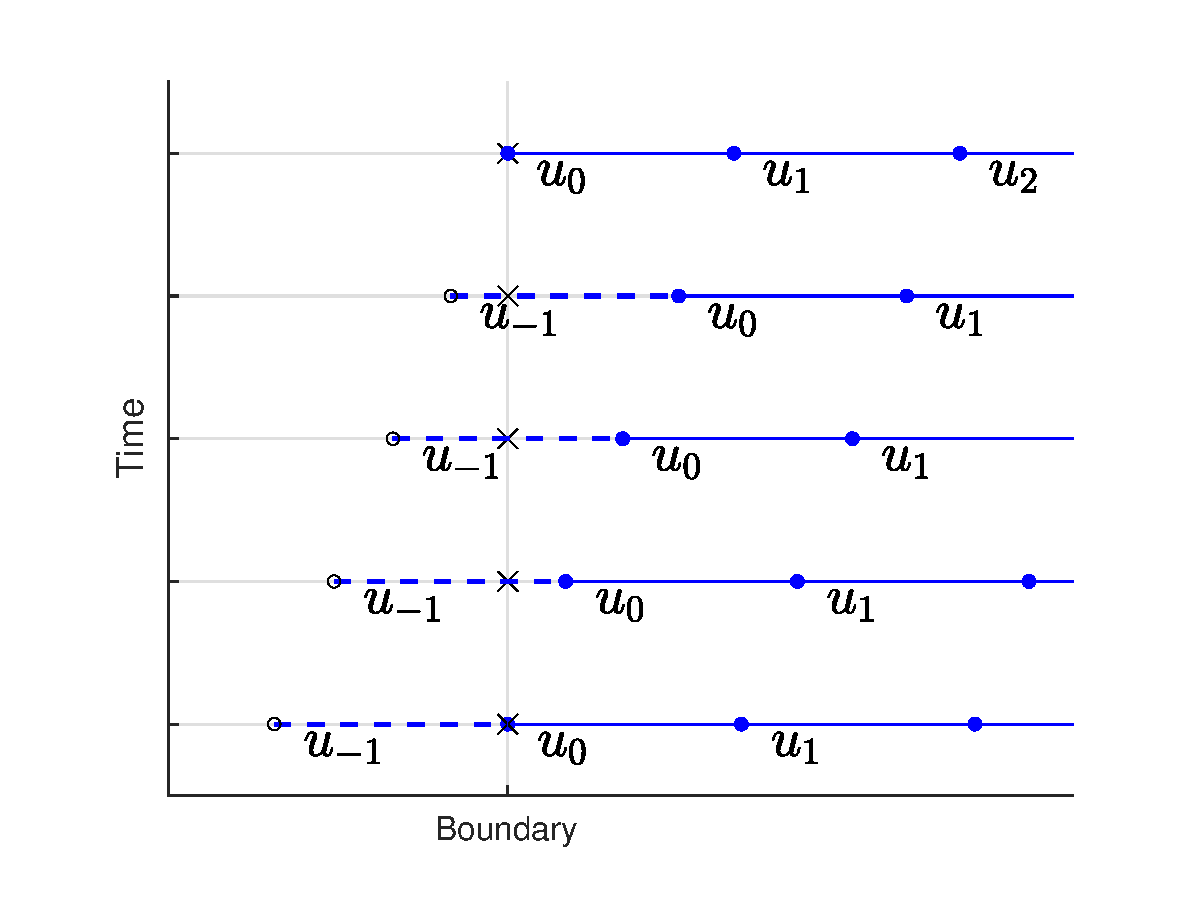
\includegraphics[width=0.7\textwidth]{dynamic/boundaryGrid.eps}
\caption{\label{fig:changingBoundary}{The grid changing over time}}
\end{figure}

\subsection{Cubic interpolation}

\subsection{Sinc interpolation}


\subsection{Displacement correction}

The displacement correction can be interpreted as a spring force pulling $u_M^n$ and $w_0^n$ to the average displacement.

\begin{align}
    &\begin{aligned}
        u_{M}^{n+1} &= 2u_M^n + \lambda^2 (u_{M-1} ^n- 2u_M^n  + u_{M+1}^n) - K \left(u_M^n - \frac{u_M^n + w_0^n}{2}\right)\\
        w_0^{n+1} &= 2u_M^n + \lambda^2 (w_{-1} ^n- 2w_0^n  + w_1^n) - K \left(w_0^n - \frac{u_M^n + w_0^n}{2}\right) 
    \end{aligned}\\
    &\begin{aligned}
        u_{M}^{n+1} &= 2u_M^n + \lambda^2 (u_{M-1} ^n- 2u_M^n  + u_{M+1}^n) + \frac{K}{2} (w_0^n - u_M^n)\\
        w_0^{n+1} &= 2u_M^n + \lambda^2 (w_{-1} ^n- 2w_0^n  + w_1^n) - \frac{K}{2} (w_0^n - u_M^n) 
    \end{aligned}
\end{align}
with $K = K(\alpha)$
\begin{equation}
    K = (1-\alpha)^\epsilon.
\end{equation}